\documentclass{standalone}
\usepackage{tikz}
\usetikzlibrary{shapes, calc}



\begin{document}


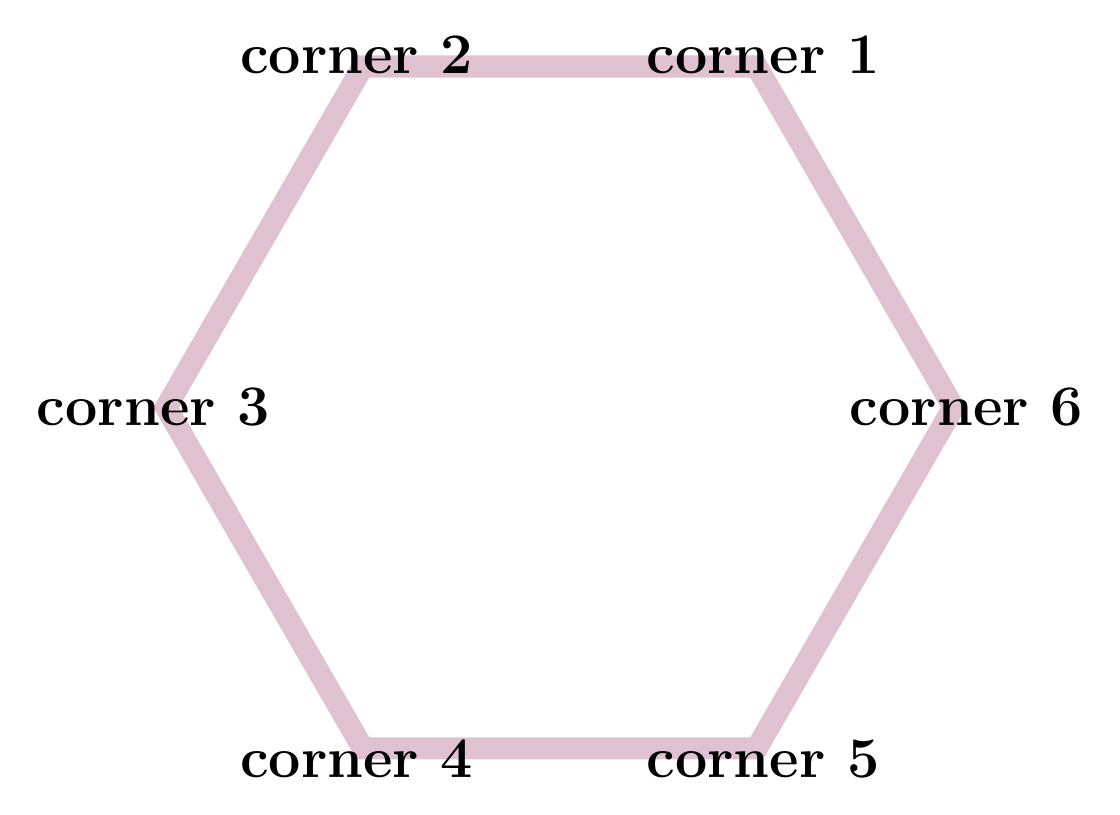
\begin{tikzpicture}[
vertex_style/.style={circle,shading=ball,ball color=red,draw=red!80!white,drop shadow={opacity=0.4}},
node_spin/.style={circle, shading=ball, ball color=gray!10!white, draw=none, minimum width=1.5cm,inner sep=0.1cm, opacity=0.7},
edge_style/.style={ultra thick, black,drop shadow={opacity=0.4}},
		hora/.style={rectangle, minimum width=1.75cm, minimum height=1.75cm, rounded corners=2mm, top color=gray!10, bottom color=brown!50}, font=\huge \bfseries, 
		]
 
\begin{scope}[xshift=0cm, rotate=0]

	\def\lados{6};
	\node[regular polygon, regular polygon sides=\lados, minimum size=10.cm, draw=purple!80!cyan, line width=8pt, transform shape, opacity=0.3] at (0,0) (polygonnode) {};

	
\foreach\i in {1,...,\lados}{
		\node[] at (polygonnode.corner \i) {corner \i};
		}
		

	
\end{scope}

\end{tikzpicture}


\end{document}
